% !TEX root = ../thesis_main.tex
\chapter{Prior Ultrafast Spectroscopy Studies of SWCNTs}

\section{Overview}

{\color{red} UNFINISHED} Want to make lasers. Need population inversion. Understood that excitons can decay in a number of processes including electron-hole recombination which results in photon emission, or through other non-radiative processes such as phonon scattering or entrapment in defects or impurities \cite{simpson1957electronic}. Not possible to achieve if nonlinear processes such as exciton-exciton annihilation or Auger scattering occur. Conflicting reports regarding whether exciton-exciton annihilation in CNTs actually occurs.


\section{Inter-band and Inter-subband Recombination Dynamics}

{\color{red} ADD INTRO PARAGRAPH FOR THIS SECTION}

Ostojic et al.\ (2004) presented an early work regarding the carrier recombination dynamics of carbon nanotubes \cite{ostojic2004interband}. They conducted wavelength-dependent, degenerate pump-probe measurements using an optical parametric amplifier with a time resolution of $\sim$150 fs (See Section \ref{section:opa} for details regarding the function of optical parametric amplifiers) whereby the pump and probe have the same photon energy. The sample they studied consisted of a dispersion of HiPCo SWCNTs (See Sections \ref{section:cnt_synthesis} and \ref{section:dispersion_swcnt} for details).

\begin{figure}[ht]
	\centering
	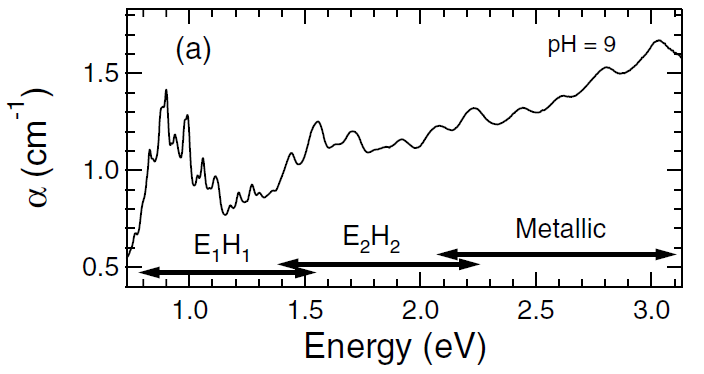
\includegraphics[scale=0.7]{images/chapter_prior_works/abs_gordana}

	\caption{Optical absorption spectrum of dispersed HiPCo SWCNTs studied by Ostojic et al.\ (2004). The spectrum contains optical resonances associated with semiconducting nanotubes which include $E_{11}$ in the region denoted as $E_{1} H_{1}$ as well as  $E_{22}$ in the region labeled as $E_{2} H_{2}$. The remaining resonances in the Metallic region come from the $E_{11}$ resonances of metallic nanotubes. Reproduced and modified from Ref.\ \cite{ostojic2004interband}.}
	\label{fig:abs_gordana}
\end{figure}


Figure \ref{fig:abs_gordana} shows the optical absorption spectrum of their sample which indicates the presence of many different chiralities, including both metallic and semiconducting nanotubes. The spectral region spanning $E_{1} H_{1}$ contains optical resonances associated with the $E_{11}$ transition occurring in semiconducting nanotubes. The region defined as $E_{2} H_{2}$ contains $E_{22}$ transitions of semiconducting nanotubes. Finally, the region defined as Metallic exhibits the remaining $E_{11}$ resonances emerging from metallic nanotubes.

\begin{figure}[ht]
	\centering
	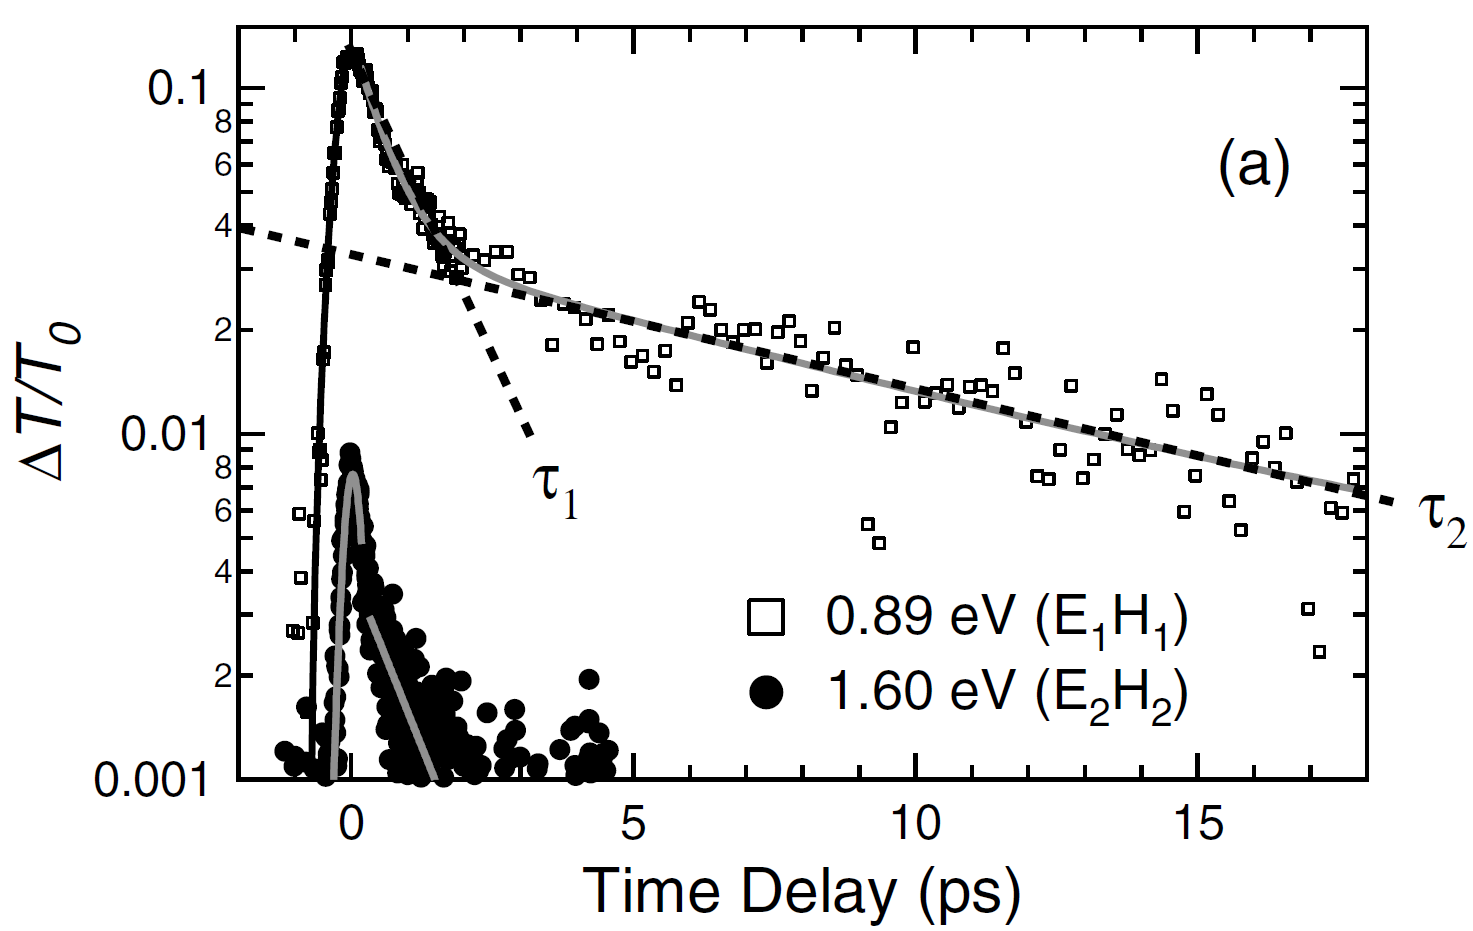
\includegraphics[scale=0.3]{images/chapter_prior_works/dtt_gordana}
	\caption{Differential transmission data at photon energies 0.89 eV (white squares) and at 1.60 eV (black circles) obtained from degenerate pump-probe measurements. At 1.60 eV, only a single exponential decay process associated with intra-band relaxation is observed. At 0.89 eV, a bi-exponential decay occurs. The fast and slow components of the bi-exponential decay are associated with intra-band and inter-band dynamics respectively. Reproduced and modified from Ref.\ \cite{ostojic2004interband}}
	\label{fig: abs_gordana}
\end{figure}

The observed carrier dynamics showed a clear wavelength dependence as shown in Figure \ref{fig:dtt_ph_gordana}. For pumping and probing within the $E_2 H_2$ region, carrier was best described by a single exponential decay process which was interpreted as intra-band relaxation to lower-energy states. In contrast, a bi-exponential decay process was observed when pumping and probing in the $E_1 H_1$ region. The initial, fast decay was interpreted as intra-band relaxation. However, the following slow exponential decay process was interpreted as inter-band relaxation. At the time of publication, this slow exponential decay process had not been observed before.

Ostojic et al.\  also note that for any chosen wavelength in their degenerate pump-probe study, some nanotubes are resonantly excited whereas others are photo-excited in a non-resonant fashion. This can affect the observed carrier decay dynamics. Figure \ref{fig:wl_dep_gordana} demonstrates this behavior. When photo-exciting the sample at an optical resonance, the ratio between the slow and fast decay times reaches a local maximum. In contrast, when pumping at spectral regions that do not exhibit a well-defined resonance, this ratio diminishes.

\begin{figure}[ht]
	\centering
	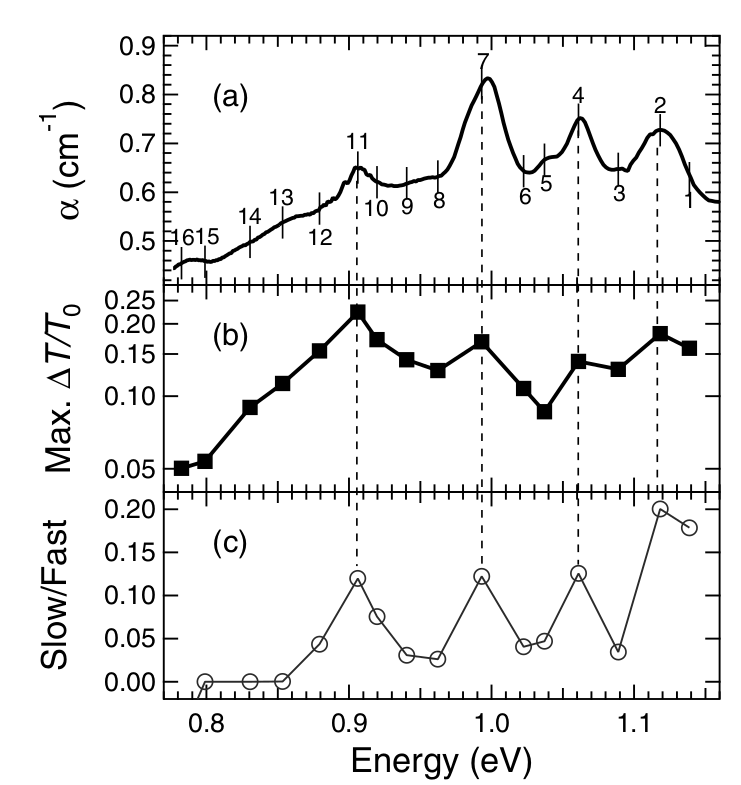
\includegraphics[scale=0.3]{images/chapter_prior_works/wavelength_dependence_gordana}
	\caption{(a) Optical absorption spectrum of the HiPCo SWCNT dispersion. The labeled positions indicate photon energies at which pump-probe measurements were taken. (b) Maximum differential transmission recorded at each measured photon energy. Differential transmission appears to reach a local maximum when the photon energy matches an optical resonance. (c) Ratio between the slow and fast decay times at each measured photon energy. The slow decay time reaches a local maximum when pumping at an optical resonance. Reproduced and modified from Ref.\ \cite{ostojic2004interband}}
	\label{fig:wl_dep_gordana}
\end{figure}

Hence, resonant excitation enhances the appearance of inter-band recombination dynamics. However, non-resonant excitations are more associated with the fast intra-band dynamics. This suggests that the reported decay times only yield statistical averages of the carrier lifetime of the ensemble of all nanotubes that have optical resonances at energies less than or equal to the pump photon energy. Furthermore, they acknowledge that they did not observe a clear correlation between the power of the optical pump and the observed carrier decay times. This excludes the observation of any nonlinear, nonradiative recombination mechanisms such as Auger recombination or exciton-exciton annihilation.

\begin{figure}[ht]
	\centering
	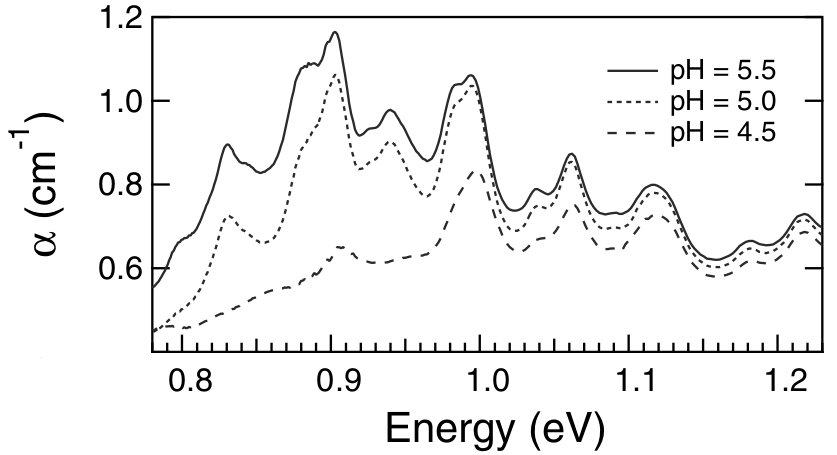
\includegraphics[scale=1.5]{images/chapter_prior_works/ph_effect_gordana_revised}
	\caption{The effect of pH on linear absorption. As the pH reduces from 5.5 to 4.5, absorption peaks at lower photon energies become supressed. This occurs as a consequence of the Burstein-Moss effect, as H$^+$ ions act as dopants that accept electrons. These dopants primarily affect larger-diameter nanotubes, as they exhibit lower binding energies for acceptors in light of their smaller effective masses. Reproduced and modified from Ref.\ \cite{ostojic2004interband}.}
	\label{fig:ph_abs_gordana}
\end{figure}

Decreasing the pH of the sample was observed to suppress optical absorption peaks, especially those occurring at lower photon energies as shown in Figure \ref{fig:ph_abs_gordana}. Correspondingly, the presence of the slow exponential decay process also diminished as shown in Figure \ref{fig:dtt_ph_gordana}. These effects were understood as a consequence of the Burstein-Moss effect. In other words, H$^+$ ions of the acidic aqueous suspension dope suspended SWCNTs by accepting negatively-charged carriers. This positions the Fermi level primarily within the valence band for nanotubes with larger diameters due to their smaller acceptor binding energies associated with their smaller effective masses.  As a result, the appearance of an inter-band absorption peak diminishes which subsequently removes the possibility of enhancing the occurrence of the inter-band relaxation by photo-exciting at well-defined optical resonances.

\begin{figure}[H]
	\centering
	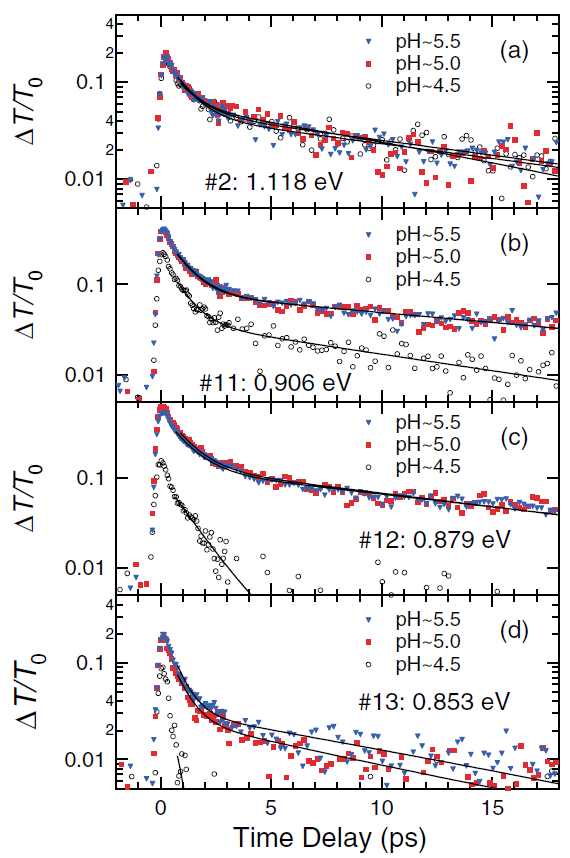
\includegraphics[scale=0.5]{images/chapter_prior_works/dtt_ph_gordana}
	\caption{The effect of pH on the carrier dynamics of nanotubes. Each plot corresponds to a degenerate pump-probe experiment conducted at a specified photon energy. As pH decreases, nanotubes become increasingly doped with positively-charge carriers. This has a larger effect on larger-diameter nanotubes due to their lower acceptor binding energies and lower the Fermi level into the valence band. At lower photon energies, the inter-band recombination process does not appear as the optical resonances associated with this process become supressed. Reproduced and modified from Ref.\ \cite{ostojic2004interband}}
	\label{fig:dtt_ph_gordana}
\end{figure}

Manzoni et al.\ (2005) investigated the inter-subband dynamics of SWCNTs using non-degenerate pump-probe measurements with a time resolution of 40 fs. They used two OPAs to generate pump and probe pulses respectively. Furthermore, the sample they studied was a nanotube film made using HiPCo SWCNTs. Figure \ref{fig:abs_manzoni} shows the optical absorption spectrum of this sample along with the specta of the pump pulses used in this study. The sample contains a variety of optical resonances that belong to semiconducting and metallic nanotubes. The spectral regions labeled as EX1, EX2, and EX3 indicate $E_{11}$, $E_{22}$, and $E_{33}$ resonances of semiconducting nanotubes respectively. The region marked as Metallic shows the $E_{11}$ resonances for metallic nanotubes.

Depending on the pump and probe photon energies, the observed carrier relaxation dynamics either exhibit photo-induced transsmission or photo-induced absorption. For instance, Figure \ref{fig:e11_pump_manzoni} shows the experimental results obtained when pumping in the EX1 region at 0.92 eV. The differential transmission signal probed at 0.95 eV shows clear signs of photo-bleaching which indicates a finite population of photo-excited carriers. In contrast, the dynamics probed at 2 eV indicate the presence of photo-induced absorption.

\begin{figure}[H]
	\centering
	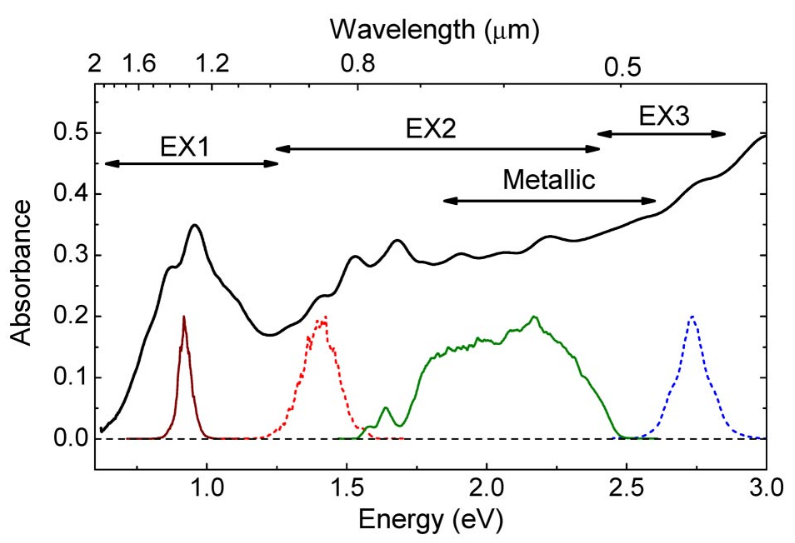
\includegraphics[scale=0.4]{images/chapter_prior_works/abs_manzoni}
	\caption{The black, solid line up top shows the absorption spectrum of HiPCo SWCNT film studied by Manzoni et al. (2005). The spectral regions indicated as EX1, EX2, and EX3 contain the $E_{11}$, $E_{22}$, and $E_{33}$ transitions of semiconducting nanotubes respectively. The region labeled as Metallic contains the $E_{11}$ resonance of metallic nanotubes. The plots shown below represent the spectra of optical pump pulses used to photo-excite the SWCNT sample in this study. Reproduced and modified from Ref.\ \cite{manzoni2005intersubband}.}
	\label{fig:abs_manzoni}
\end{figure}

Photo-bleaching does not occur due to the fact that the photon energy of the pump is below photon energies of the resonances in EX2. Hence, this photo-induced absorption was interpreted to occur due to an inter-subband transition between a state in the EX1 region and another appropriate state located in EX3 as the energy difference between two such states would be on the order of 2 eV. Additionally, this probe signal at 2 eV exhibits an oscillatory component that was attributed to a radial breathing mode (RBM) of semiconducting CNTs that occurs at a frequency of 259 $\text{cm}^{-1}$. From examining Raman spectra, this indicated that SWCNTs such as (10,3), (11,1), (9,4) and (9,4) were photo-excited in this measurement.


When exciting the SWCNTs at an energy of 2.15 eV in the EX2 region, different dynamics occurred as shown in Figure \ref{fig:e22_pump_manzoni}. Photo-bleaching occurred at the probed photon energy of 0.95 eV. In addition, both photo-induced and transmission and absorption occurred at the probed photon energy of 2.15 eV. The initial photo-bleaching indicates a finite population of $E_{22}$ excitons. Furthermore, the decay occuring afterwards indicates the relaxation from $E_{22}$ to $E_{11}$. This process occurs on a time scale of 150 fs with an associated exponential decay constant of $\sim$40 fs. The photo-induced absorption was again interpreted to occur due to a possible transition between an EX1 state and an EX3. An oscillatory signal was also observed here which was associated with an RBM frequency of 246 $\text{cm}^{-1}$ linked with nanotubes such as (10,3), (9,5), (9,4), and (7,6).


Figure \ref{fig:e33_pump_manzoni} illustrates the effect of photo-exciting at 2.75 eV (EX3) and probing at 2.1 eV (EX2). Under these conditions, a small photo-bleaching signal followed by photo-induced absorption occurred. This demonstrated the fast relaxation dynamics from EX3 states into EX1 states. Furthermore, the time constant for this process found to be $\sim$65 fs. Following the previous observations, the photo-induced absorption observed at EX2 also indicated the carrier occupation of EX1 states.

Finally, Manzoni et al.\ mentioned that they observed a weak relationship between optical pump intensity and observed recombination dynamics as shown in the inset plot of Figure \ref{fig:e22_pump_manzoni}. At higher pump intensities, the time constant for the exponential decay did not change in a significant fashion. Thus, they did not observe exciton-exciton annihilation in their studies.

\begin{figure}[H]
	\centering
	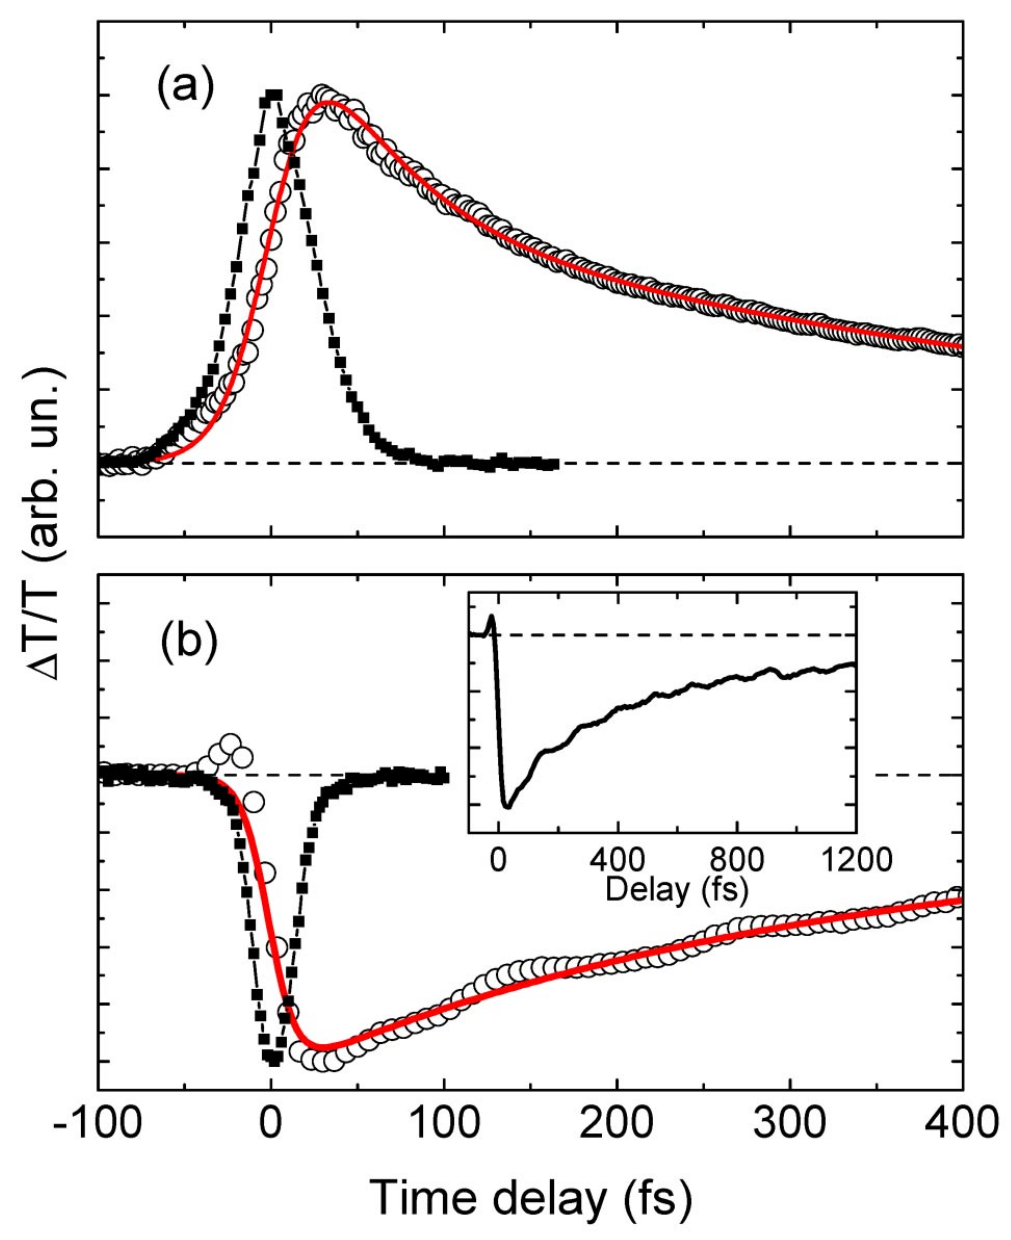
\includegraphics[scale=0.2]{images/chapter_prior_works/e11_pump_probe_manzoni}
	\caption{Carrier relaxation dynamics of SWCNTs photo-excited at 0.92 eV. Under this condition, the two plots correspond to differential transmission probed at 0.92 eV (a) and probed at 2.15 eV (b). The inset figure shows the relaxation measured at 2 eV on a longer time scale. The open circles represent the experimental data, and the solid lines indicate numerical fits to the data. The autocorrelation measurement of the pump pulse is also overlayed on both figures (squares + line). Reproduced from Ref.\ \cite{manzoni2005intersubband}.}
	\label{fig:e11_pump_manzoni}
\end{figure}

\begin{figure}[H]
	\centering
	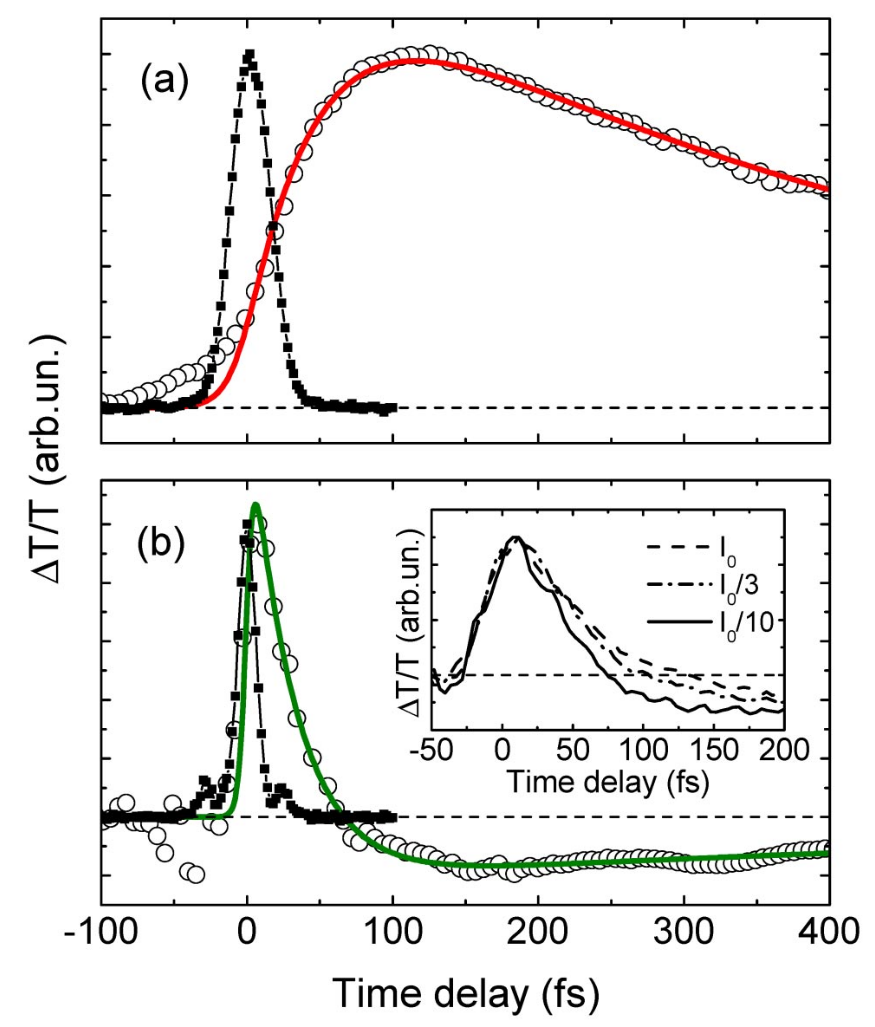
\includegraphics[scale=0.25]{images/chapter_prior_works/e22_pump_probe_manzoni}
	\caption{Carrier relaxation dynamics of SWCNTs photo-excited at 2.15 eV. Under this condition, the two plots correspond to differential transmission probed at 0.95 eV (a) and probed at 2 eV (b). The inset figure shows the pump power dependence measurements of the differential transmission probed at 2 eV. The open circles represent the experimental data, and the solid lines indicate numerical fits to the data. The autocorrelation measurement of the pump pulse is also overlayed on both figures (squares + line). Reproduced from Ref.\ \cite{manzoni2005intersubband}.}
	\label{fig:e22_pump_manzoni}
\end{figure}

\begin{figure}[ht]
	\centering
	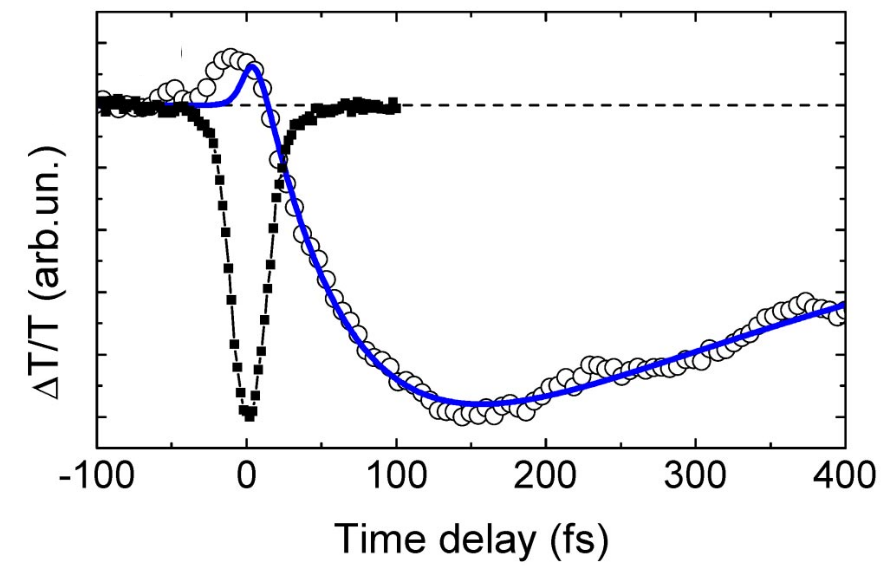
\includegraphics[scale=1.3]{images/chapter_prior_works/e33_pump_e22_probe_manzoni}
	\caption{Carrier relaxation dynamics of SWCNTs photo-excited at 2.75 eV and probed at 2.1 eV. The open circles represent the experimental data, and the solid line indicates a numerical fit to the data. The autocorrelation measurement of the pump pulse is also overlayed on the plot (squares + line). Reproduced from Ref.\ \cite{manzoni2005intersubband}.}
	\label{fig:e33_pump_manzoni}
\end{figure}


In general, excitons are expected to be stable in a scenario where their Bohr radius $r_\text{Bohr}$ is much smaller than the typical inter-exciton distance $d_\text{exc}$ \cite{mott1961transition}. Increasing the density of excitons can establish a condition where
\begin{equation}
r_\text{Bohr} \approx d_\text{exc},
\end{equation}
once the density is greater than or equal to a critical value known as the Mott density \cite{mott1961transition}. This causes a Mott transition process to occur where screening effects suppress the Coulomb interaction between electrons and holes, causing them to dissociate to create a free electron plasma \cite{mott1961transition}. Ostojic et al.\ (2005) investigated this phenomenon in SWCNTs using non-degenerate, pump-probe spectroscopy \cite{ostojic2005stability} featuring a broadband probe. They claim that even at the Mott density, excitons still remain stable.

\begin{figure}[ht]
	\centering
	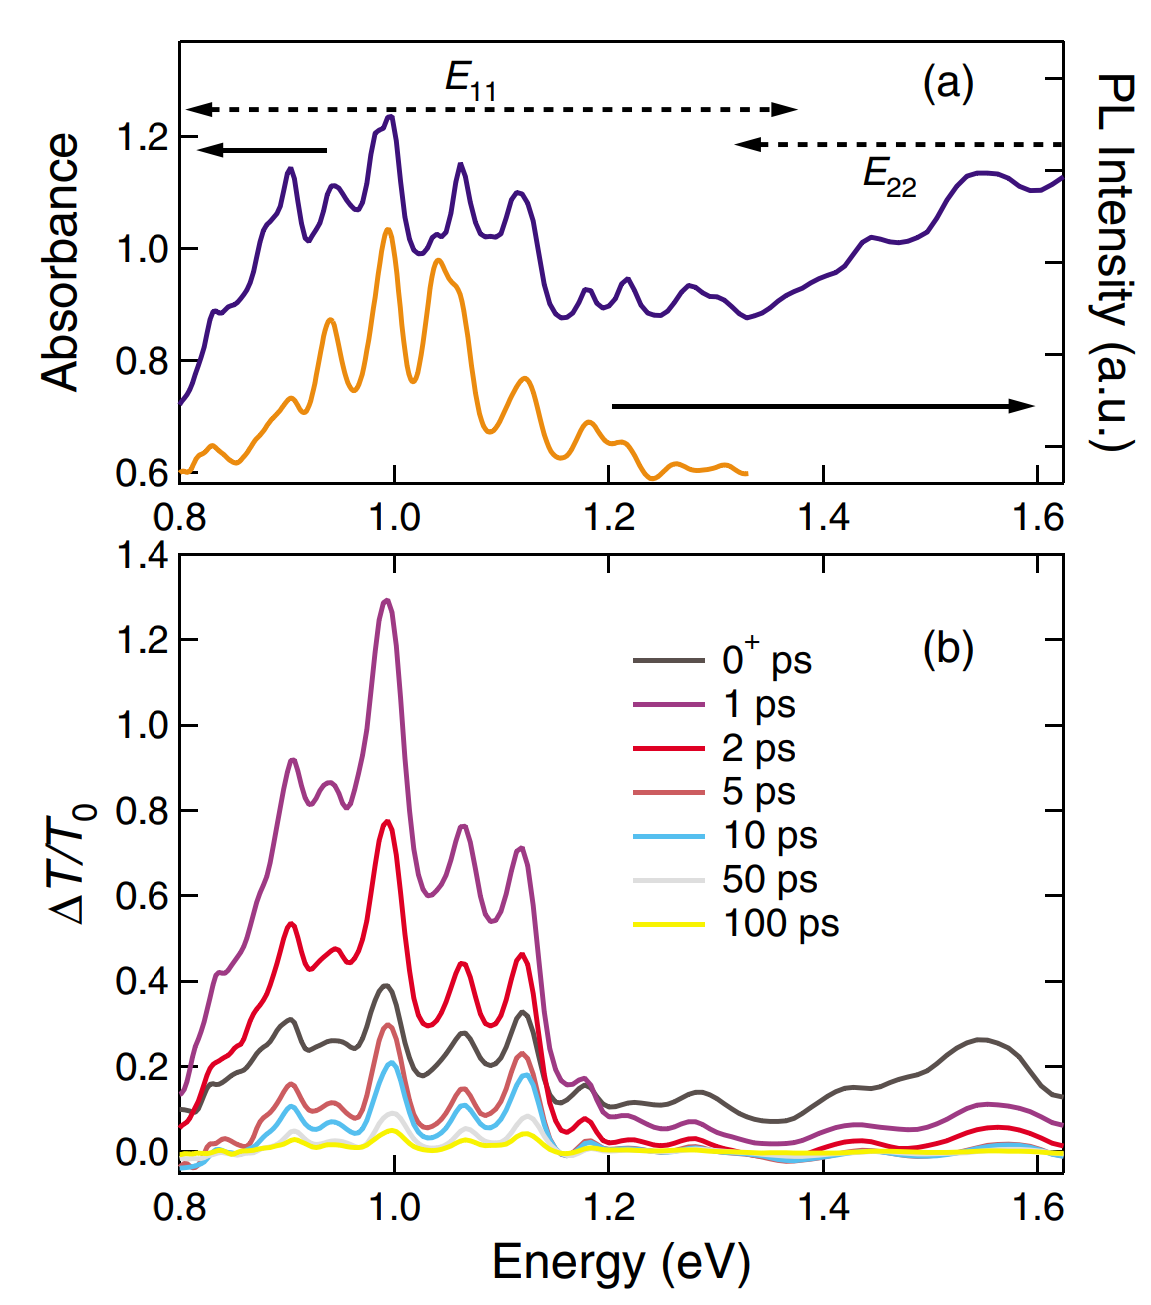
\includegraphics[scale=0.22]{images/chapter_prior_works/abs_dtt_gordana_2005}
	\caption{{\color{red} UNFINISHED} Reproduced from Ref.\ \cite{ostojic2005stability}. }
	\label{fig:abs_dtt_gordana_2005}
\end{figure}

Figure \ref{fig:abs_dtt_gordana_2005} shows the linear absorption and photoluminescence spectra of their HiPCo SWCNT dispersion sample as well as differential transmission data obtained at various time delays. The differential transmission data was taken using an optical pump centered at \SI{775}{\nano\meter}. Within the first \SI{1}{\pico\second}, the signal observed within the $E_{22}$ range appears to decay whereas, that of the $E_{11}$ range increases rapidly. This agrees with the fast inter-subband dynamics observed by Manzoni et al.\ (2005). Moreover, the spectral shape of the differential transmisson stays constant and only changes in amplitude.


\begin{figure}[ht]
	\centering
	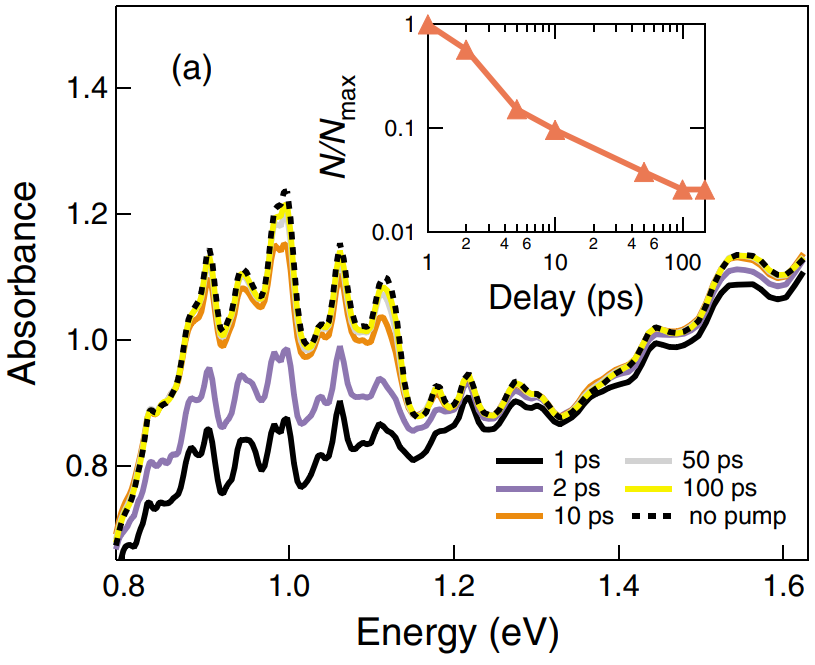
\includegraphics[scale=1.2]{images/chapter_prior_works/total_abs_gordana_2005}
	\caption{{\color{red} UNFINISHED} Reproduced from Ref.\ \cite{ostojic2005stability}.}
	\label{fig:total_abs_gordana_2005}
\end{figure}


These effects can be interpreted more easily by taking the linear absorption of the sample into account. Hence, Figure \ref{fig:total_abs_gordana_2005} shows how the total absorbance of the sample changes. The absorption associated with excitonic resonances decreases due to photo-bleaching effects. However, the overall shape of these resonances appears t remain constant. The peak positions do not shift in energy either.

Ostojic et al.\ (2005) estimate the number of photo-excited excitons in nanotubes by taking into account the total number of nanotubes within the photo-excited volume of their sample, the change in absorbance, as well as the pump fluence. They deduce that the density of excitons in a typical nanotube of length \SI{150}{\nm} is on the order of $5 \times 10^6$ \si{\per\cm}. This yields an average seperation of \SI{2}{\nm} between excitons. In addition, they acknowledge that theoretical calculations in the literature that suggest that the typical Bohr radius in SWCNTs of diameter 1 nm range between 2 - 5 \si{\nm}.

Estimates such as these imply that that shortly after photoexcitation, the optical pump creates enough excitons such that a Mott transition may indeed occur as the Bohr radius is of the same order of magnitude as the average inter-exciton distance. However, the presence that exciton resonances even at high pump fluences shows that excitons have not yet dissociated to form a free-electron plasma. Experimental results such as these have raised questions as to whether it is even possible to reach the Mott density in SWCNTs. Indeed, a number of studies have presented evidence that efficient exciton-exciton annihilation processes in SWCNTs establish an upper limit on the density of excitons that is below the Mott density.


\section{Exciton-Exciton Annihilation}



{\color{red} ADD INTRO PARAGRAPH FOR THIS SECTION}

First explored by Northrop et al.\ as a means of explaining transport properties of molecular crystals \cite{northrop1958electronic}.

\begin{equation}
\label{eq:exc_annih}
\ce{2 $E_{x_1}$ $\rightarrow$  $E_{x_2}$ + $GS$ \rightarrow $E_{x_1}$ + $GS$},
\end{equation}

where $E_{x_1}$, $E_{x_2}$, reprsent first and second sub-bands of the conduction band respectively and $GS$ is the ground state.
\begin{equation}
	\frac{\partial n(\vec{r}, t)}{\partial t} = - \gamma n(\vec{r}, t)^2
\end{equation}

Without exciton-exciton annihilation, dynamics of carrier relaxation should linearly depend on fluence of optical pump.

\subsection{Early Evidence in Support of Exciton-Exciton Annihilation}
{\color{red} UNFINISHED}
Wang et al.\ (2004) observed non-linear recombination dynamics in time-resolve fluorescence experiments \cite{wang2004observation}. Measured a dispersion of HiPco SWCNTs. Figure \ref{fig:fluorescence_wang_2004} shows results. At higher pump fluences, the onset of a fast exponential decay process becomes more prominent. This behavior exemplifies a well-known signature of Auger recombination processes. In addition, the fluorescence observed at longer time delays appears to saturate as shown in the inset plot of Figure \ref{fig:fluorescence_wang_2004}.



Furthermore, Figure \ref{fig:fast_slow_wang_2004} shows the time-integrated fluoresence contributions associated with the fast and slow decays. The fluorescence from the slow decay begins saturating at fluences greater than \SI{0.3}{\joule / \meter\squared}. In contrast, the time-integrated fluoresence linked with the fast decay only begins to saturate at a fluence of \SI{1.5}{\joule / \meter\squared}. These data suggest that exciton-exciton annihilation associated with the fast decay process establishes an upper limit of bright excitons that can exist at longer time delays.

\begin{figure}[H]
	\centering
	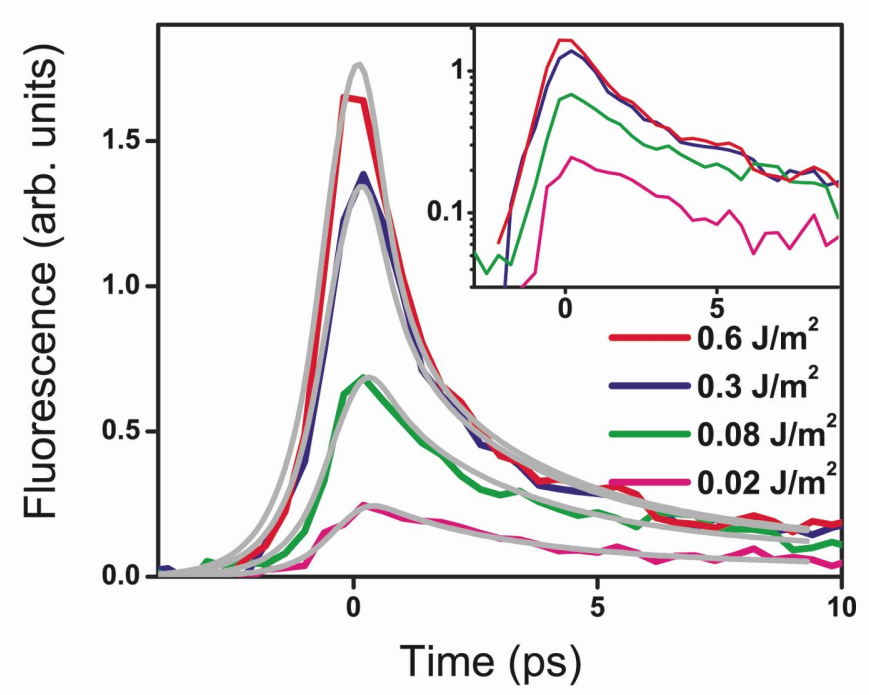
\includegraphics[scale=0.25]{images/chapter_prior_works/fluorescence_wang_2004}
	\caption{Time-resolved fluorescence captured at indicated fluences. The optical pump pulse was centered 810 nm. Gray curves are fits to the experimental data using a model based on exciton-exciton annihilation. At higher fluences, the dynamics exhibit a bi-exponential decay containing a fast and a slow process. The fast exponential decay has been attributed to the presence of a non-radiative decay mechanism associated with exciton-exciton annihilation whereas, the slow component emerges due to radiative inter-band recombination. The inset figure shows the same experimental data on a log-linear plot to emphasize the saturation of the fluoresence at higher pump fluences occuring due to non-radiative decay phenomena. Reproduced from Ref.\ \cite{wang2004observation}.}
	\label{fig:fluorescence_wang_2004}
\end{figure}



Wang et al.\ interpreted these results by devising a model of carrier dynamics that accounts for Auger recombination processes. They postulate that the time-dependent, probability distribution of a nanotube having $N$ electron-pairs $\rho^\text{N}(t)$ depends on the rate of radiate emission $\gamma^\text{N}_\text{r}$, the rate of Auger recombination $\gamma^\text{N}_\text{A}$, as well as the rate of carrier trapping at defects $\gamma_\text{t}$. The master equation
\begin{equation}
	\dfrac{\mathrm{d}\rho^\text{N}}{\mathrm{d} t} = \rho^\text{N}(\gamma^\text{N+1}_\text{r} + \gamma^\text{N+1}_\text{A} + \gamma_\text{t})(N+1) - \rho^\text{N}(\gamma^\text{N}_\text{r} + \gamma^\text{N}_\text{A} + \gamma_\text{t})N,
\end{equation}
captures the relationship between these quantities. In the case of excitons,
\begin{equation}
	\gamma^\text{N}_\text{r} = \text{const}, \text{   } \gamma^\text{N}_\text{A} = C_\text{A}(N-1),
\end{equation}
where $C_\text{A}$ is the Auger rate coefficient. Initial population of excitons $N_\text{initial} = \phi \sigma$, where $\phi$ and $\sigma$ denote, respectively, the fluence of the optical pump and the absorption cross-section of carbon nanotubes. Indeed the qualitative results from this model agree with the experimental data presented in Figures \ref{fig:fluorescence_wang_2004} and \ref{fig:fast_slow_wang_2004}.



Numerical fits to the data yield an estimate of $C_\text{A}$ which was found to be $\SI{0.8}{\per\pico\second}$. Correspondingly, this also provides an estimate of the typical lifetime of excitons that participate in exciton-exciton annihilation given as $1/\gamma^\text{N}_\text{A}$ which was determined to be on the order of picoseconds with lifetimes being as short as \SI{1.2}{\pico \second}.




\begin{figure}[ht]
	\centering
	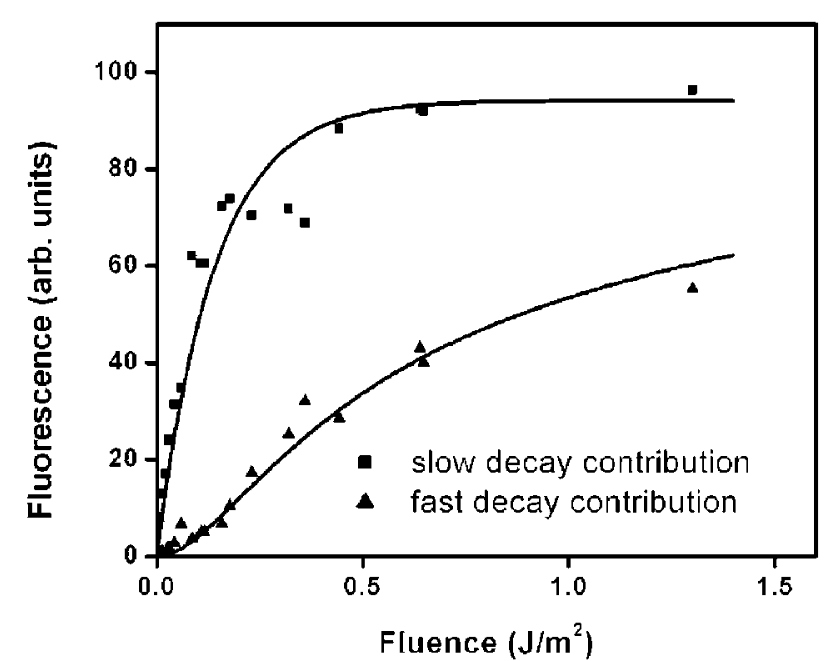
\includegraphics[scale=0.3]{images/chapter_prior_works/fast_slow_wang_2004}
	\caption{Time-integrated fluorscence associated with fast and slow decay contributions as a function of pump fluence. The solid curves represent fits to the data. The fluorescence associated with the slow decay saturates at a fluence above \SI{0.3}{\joule / \meter \squared}, indicating an upper limit of bright excitons. However, the time-integrated fluorescence of the fast decay only begins to saturate at 1.5  \SI{1.5}{\joule / \meter \squared}. Reproduced from Ref.\ \cite{wang2004observation}.}
	\label{fig:fast_slow_wang_2004}
\end{figure}

Ma et al.\ (2004) also obtained some experimental results that qualtitatively agree with those observed by Wang et al (2004). In this work, they performed both time-resolved fluorescence as well as time-resolved transient absorption measurements on a HiPCo SWCNT dispersion. Figure \ref{fig:fluorescence_ma_2004} shows the fluorescence of (9,5) nanotubes that occurred after resonantly photo-exciting at the $E_{22}$ energy. As the intensity of the optical pump increases, the presence of an early fast decay processes becomes more prominent close to time zero.
%

%
Here, Ma et al.\ used the rate equation
\begin{equation}
	\dfrac{\mathrm{d}N(t)}{\mathrm{d}t} = - k N(t) - \gamma N(t)^2,
\end{equation}
to characterize the observed carrier dynamics. Here, $N$ denotes the average number of excitons at the $E_{11}$ energy level. The constants $k$ and $\gamma$ refer to the linear exciton decay rate, as well as the exciton-exciton annihilation rate respectively. If $kt < 1$, this gives the analytical solution
\begin{equation}
	N(t) = \dfrac{N(0)}{1 + N(0)\gamma \cdot t},
\end{equation}
where $N(0)$, a fitting parameter, yields the initial population of excitons. Furthermore, the assumption that the time-dependent, fluorescence intensity $I(t)$ is proportional to $ N(t)$ gives the expression
\begin{equation}
  	\left( \dfrac{I(t)}{I_0} \right)^{-1} \approx \left( \dfrac{N(t)}{N_0} \right)^{-1} = \gamma N(0) \cdot t + 1
\end{equation}
%The results obtained from transient absorption measurements appear to exhibit some key differences from those obtained in the fluorescence measurements.
This suggests that the reciprocal of $I(t)$ has a linear dependence on time $t$. Indeed, this shows good agreement with the data as shown in Figure \ref{fig:fluorescence_abs_ma_2004}(c) except at longer time delays for higher pump fluences.

\begin{figure}[H]
	\centering
	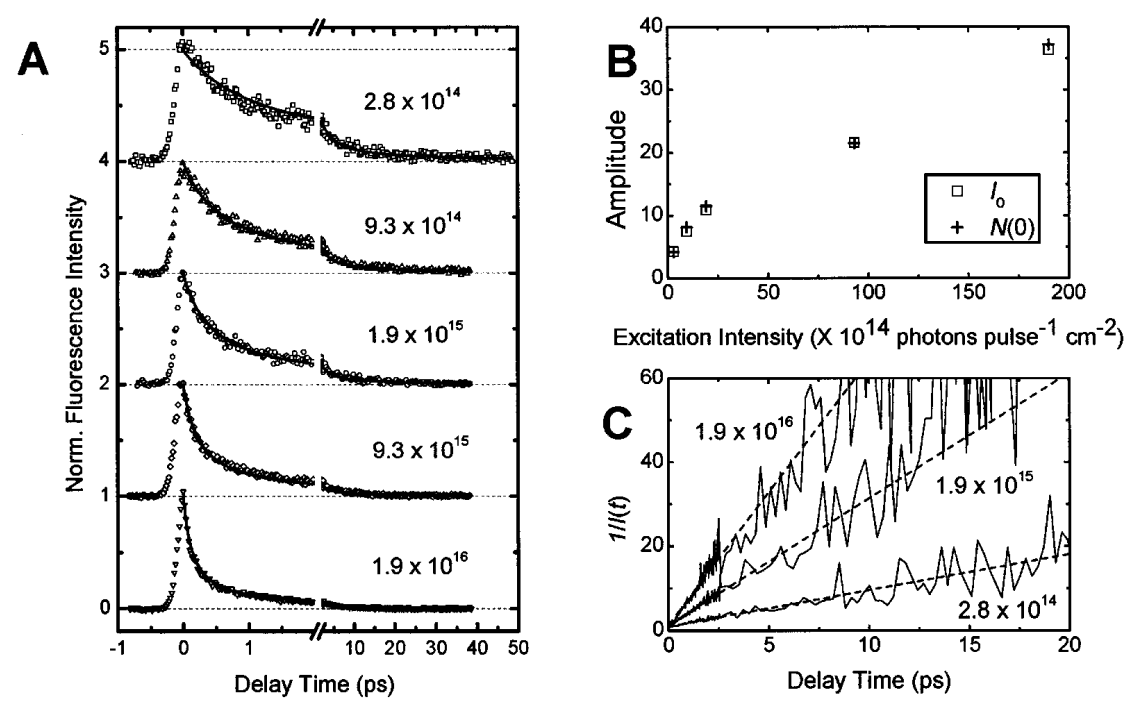
\includegraphics[scale=0.35]{images/chapter_prior_works/fluorescence_2_ma_2004}
	\caption{(a) Normalized time-resolved fluorescence measurements obtained from (9,5) nanotubes after exciting the $E_{22}$ resonance at different excitation fluences (photons\si{/\cm \squared}). At higher fluences, a fast decay component becomes more prominent. Solid lines represent fits to the data. (b) The maximum fluoresence intensity $I_0$ measured at each excitation fluence, along with the fitted parameter N(0). (c) The reciprocal of the fluorescence intensity taken at the labeled fluences and plotted as a function of time. The dashed lines represent fits to the data. Reproduced and modified from Ref.\ \cite{ma2004ultrafast}.}
	\label{fig:fluorescence_ma_2004}
\end{figure}

Figure \ref{fig:fluorescence_abs_ma_2004} shows more fluorescence and transient absorption measurements obtained from (6,5) and (7,5) nanotubes. More specifically, Figure \ref{fig:fluorescence_abs_ma_2004}(a) shows the fluorescence obtained from (6,5) nanotubes after resonantly exciting at $E_{22}$ photon energy. The results qualitatively match those of Figure \ref{fig:fluorescence_ma_2004}(a). However, the transient absorption data taken from (6,5) and (7,5) nanotubes after resonantly exciting their $E_{22}$ resonances and probing the dynamics at their respective $E_{11}$ energies appears to show some different carrier dynamics.

For the case of (6,5) nanotubes, Ma et al.\ observed that the transient absorption curves show a weaker dependence on the pump intensity at fluences less than $2 \times 10^{15}$ photons/cm$^2$. This of course contrasts with the fluorescence data which shows a substantial pump intensity dependence at all reported fluences. Moreover, they also observe some key differences between the transient aborption data taken for (6,5) and (7,5) nanotubes. In particular, when probing the $E_{11}$ resonance of (6,5) nanotubes, the transient absorption exhibits an early decay that becomes faster at higher fluences. However, for (7,5) nanotubes this early decay instead becomes slower at higher excitation intensities.

These key differences lead Ma et al.\ to conclude that a different set of carrier relaxation processes may be contributing the transient absorption dynamics. In the case of (7,5) nanotubes, they interpreted that excitons may become trapped or even convert to triplet states. For (6,5) nanotubes, they suggested that the fluence threshold of $2 \times 10^{15}$ photons/cm$^2$ needed to observe clear nonlinear dynamics indicates that other than bright excitons, the probe may also be detecting the presence of unbound electron-hole pairs.

\begin{figure}[H]
	\centering
	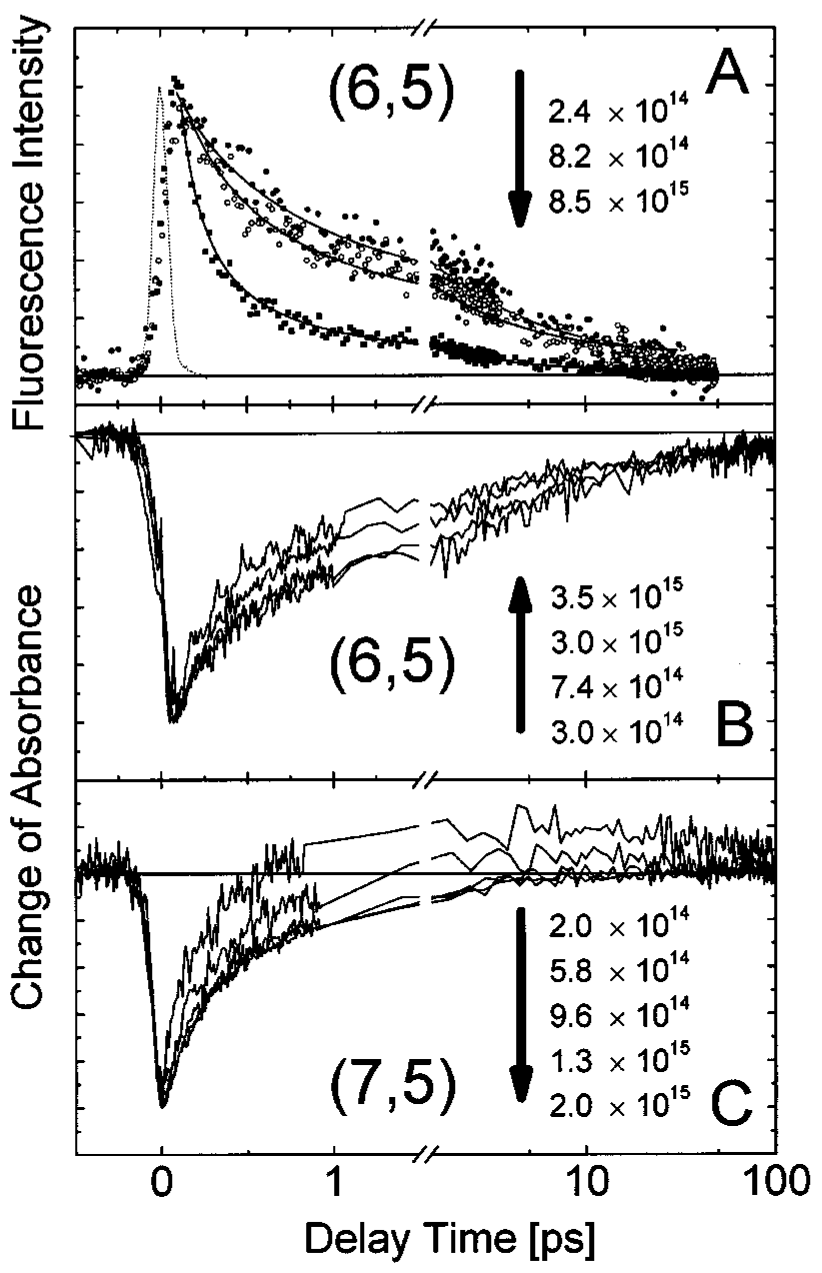
\includegraphics[scale=0.3]{images/chapter_prior_works/fluorescence_abs_2_ma_2004}
	\caption{(a) Time-resolved fluorescence measurements  obtained from (6,5) nanotubes after resonantly exciting the $E_{22}$ state at the reported fluences (photons\si{/\cm \squared}). The dynamics show a clear dependence on intensity at all fluences. (b) Transient absorption data probed at the $E_{11}$ energy (6,5) carbon nanotubes after photo-exciting the $E_{22}$ resonance at the reported fluences. These show a weak pump intensity dependence at fluences below $2 \times 10^{15}$ photons/cm$^2$. The early decay also becomes faster at higher fluences. (c) Transient absorption data probed at the $E_{11}$ energy (7,5) carbon nanotubes after photo-exciting the $E_{22}$ resonance at the reported fluences. The early decay becomes much slower at higher pump fluences. Reproduced from Ref.\ \cite{ma2004ultrafast}.}
	\label{fig:fluorescence_abs_ma_2004}
\end{figure}

In a follow-up work, Ma et al.\ (2005) measured transient absorption dynamics of (8,5) carbon nanotubes contained within a dispersion of HiPCo SWCNTs \cite{ma2005femtosecond}. In this case, they attempted to account for the carrier dynamics occuring at both the $E_{11}$ and the $E_{22}$ energy levels. Figure \ref{fig:exciton_schematic_ma} presents a schematic diagram of this approach. In this notation, each sub-band denoted as $E_i(\mathbf{k})$ contains $n_\text{i}$ excitons. Excitons at the lowest sub-band conduct exciton-exciton annihilation at rate $\gamma n_1^2/2$ which subsequently populates higher energy sub-bands. Finally, $k_\text{ij}$ represents linear relaxation rates from the $i$-th sub-band to the $j$-th sub-band and $k_\text{1g}$ measures the relaxation rate from $E_i(\mathbf{k})$ to the ground state.

\begin{figure}[ht]
	\centering
	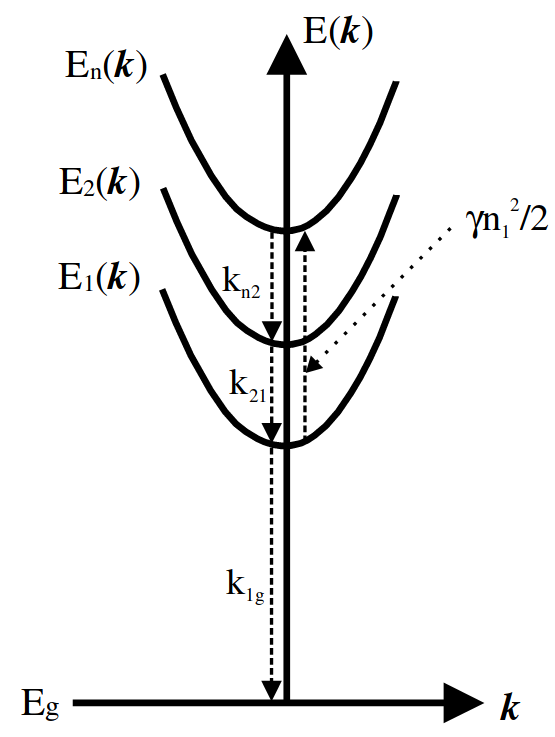
\includegraphics[scale=0.3]{images/chapter_prior_works/exciton_schematic_ma_2005}
	\caption{{\color{red} UNFINISHED} Reproduced from Ref.\ \cite{ma2005femtosecond}.}
	\label{fig:exciton_schematic_ma}
\end{figure}

After assuming that the relaxation rates $k_\text{n2}$ and $k_\text{21}$ are very fast, Ma et al. deduce that
\begin{equation}
	n_2(t) \cong \frac{1}{2 k_{21}} \gamma n^2_1(t),
	\label{eq:ma_n2}
\end{equation}
where exciton-exciton annihilation in the $E_1(\mathbf{k})$ sub-band quickly creates a population of excitons in the $E_2(\mathbf{k})$ sub-band. Furthermore, they also state that
\begin{equation}
\frac{\mathrm{d} n_1(t)}{\mathrm{d}t} = G(t) - \frac{1}{2}\gamma n_1^2(t) - k_\text{1g} n_1(t),
\end{equation}
where G(t) represents the generation rate of excitons.  This yields a formal solution which can be written as
%
\begin{equation}
	n_1(t) = \frac{n_1(0)e^{-k_\text{1g}t}}{1 + n_1(0) \gamma\cdot(1 - e^{-k_\text{1g}t} )/2k_\text{1g}}.
	\label{eq:exciton_anih_ma_2005}
\end{equation}
%

Equation \eqref{eq:ma_n2} indicates that $n_2(t) \propto n_1^2(t)$. Indeed, the experimental data shown in Figure \ref{fig:abs_ma_2005}(a) appears to corroborate this. This plot shows the transient absorption response of (8,5) nanotubes probed at $E_{11}$ (953 nm) and $E_{22}$ (660 nm) states after resonantly exciting at the $E_{11}$ photon energy. The square of the normalized transient absorption response measured at $E_{11}$ matches the dynamics of the normalized response recorded at $E_{22}$.

\begin{figure}[ht]
	\centering
	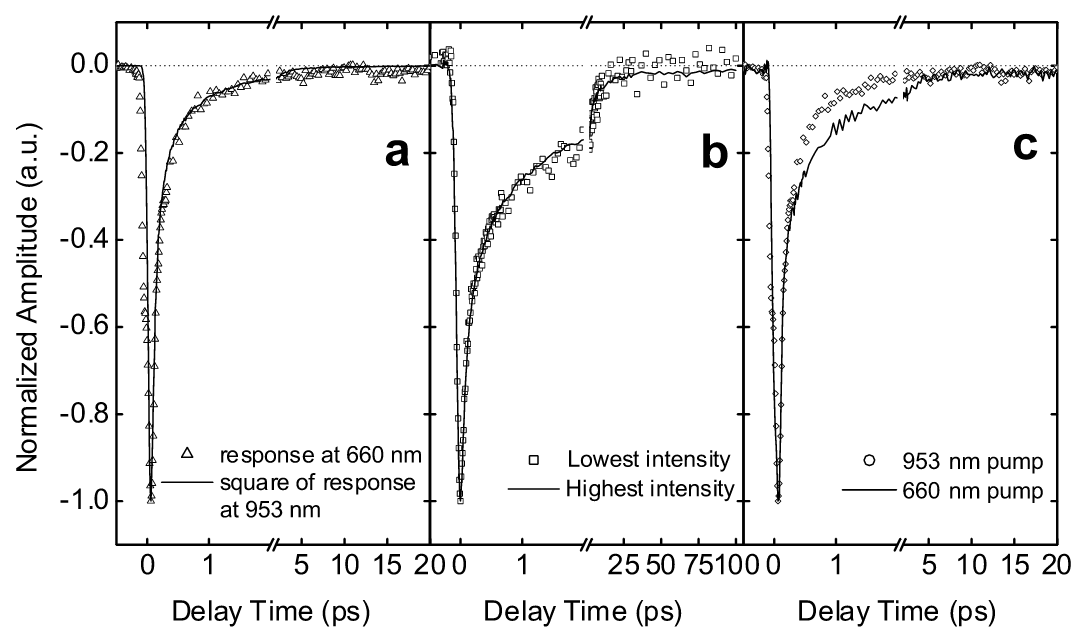
\includegraphics[scale=0.35]{images/chapter_prior_works/abs_ma_2005}
	\caption{{\color{red} UNFINISHED} Reproduced from Ref.\ \cite{ma2005femtosecond}.}
	\label{fig:abs_ma_2005}
\end{figure}

Strangely, they did not observe nonlinear carrier relaxation dynamics occuring at $E_{11}$ after resonantly exciting at $E_{11}$. Figure \ref{fig:abs_ma_2005}(b) demonstrates this. Both transient absorption curves taken at the highest and lowest fluences, which differ by a factor of 17, show similar decay rates. Also, they do acknowledge that Equation \eqref{eq:exciton_anih_ma_2005} provides good fits to the data, but only at very early times where $k_\text{1g} t \ll 1$ and for relatively high excitation fluences. Under these conditions, Equation \eqref{eq:exciton_anih_ma_2005} becomes
\begin{equation}
		n_1(t) = \frac{e^{-k_\text{1g}t}}{\gamma\cdot(1 - e^{-k_\text{1g}t} )/2k_\text{1g}}.
\end{equation}
However, a second exponental decay must be added to describe dynamics occuring at longer time delays. They attribute this to carrier dynamics detected from other nanotube species in the sample.

 Figure \ref{fig:abs_ma_2005}(c)

\subsection{Diffusion-Limited, Exciton-Exciton Annihilation}
{\color{red} UNFINISHED} The previous works presenting evidence of exciton-exciton annihilation relied on models that did not explicitly account for a key detail: the ratio between the Bohr radius of excitons and the size of the system, that is, the length scales of SWCNTs. In fact, exciton-exciton annihilation can exist in two regimes \cite{valkunas2006exciton}. On one hand, if exciton sizes are comparable to that of the system then the exciton-exciton annihilation rate should only depend on the rate at which two neighboring excitons interact with each other \cite{valkunas2006exciton}. On the other hand, if excitons are much smaller than the system they inhabit, then excitons must migrate until they reach another exciton before exciton-exciton annihilation occurs \cite{valkunas2006exciton}. In this case, the rate of exciton-exciton annihilation depends on both the diffusion rate of excitons as well as the annihilation rate of excitons in close proximity with each other \cite{valkunas2006exciton}. Hence, this regime is often referred to as diffusion-limited, exciton-exciton annihilation.

The rate of diffusion processes certainly depends on the dimensionality $d$ of the system. In fact, the decay constant associated with exciton-exciton annihilation is time-independent only in cases where $d \geq 2$ \cite{valkunas2006exciton}. For one-dimensional systems, the annihilation rate assumes the form $\gamma = \gamma_0 / t^{-1/2}$ and yields the rate equation
\begin{equation}
		\frac{\mathrm{d} n_\text{ex}^2(t)}{\mathrm{d}t} = -\frac{1}{2 \sqrt{t}}  \gamma_0 \cdot n_\text{ex}^2(t).
		\label{eq:exc_1d_annih}
\end{equation}
 This is rooted in the fact that a particle executing a random walk in three dimensions will return to its origin position with a probabilty of 0.35, whereas in dimensions less than or equal to 2 this probability is approximately unity \cite{suna1970kinematics}. As a result, the decay constant reduces with time.

The solution to this revised rate equation is then given as
\begin{equation}
	\frac{n_\text{ex}(0)}{n_\text{ex}(t)} = 1 + n_\text{ex}(0) \gamma_0 \sqrt{t},
\end{equation}
which does not fit experimental data very well. For this reason Valkunas et al.\ argued that diffusion-limited, exciton-exciton annihilation is not the correct interpretation of the results. They claimed that it must be the case that exciton sizes are on the order of typical nanotube lengths so the effects of diffusion ought to be negligible. As a result, they modeled carrier dynamics using a scheme depicted in Figure \ref{fig:exciton_manif_valkunas}. Two sets of electronic states: those that couple directly to light and those that do not. From this, they derive a set of rate equations. Solving this gives dynamics that they claim fit the data well.


\begin{figure}[ht]
	\centering
	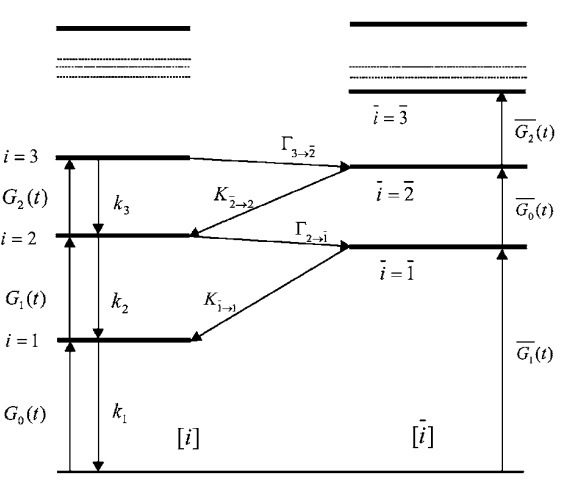
\includegraphics[scale=0.5]{images/chapter_prior_works/exciton_manifold_valkunas_2006}
	\caption{ {\color{red} UNFINISHED} Reproduced from Ref.\ \cite{valkunas2006exciton}. }
	\label{fig:exciton_manif_valkunas}
\end{figure}

{\color{red} UNFINISHED} In contrast with this, Luer et al.\ (2009) provided experimental evidence showing that exciton-exciton annihilation in SWCNTs is indeed diffusion-limited and can be modeled using the appropriate 1-D decay constant presented in Equation \eqref{eq:exc_1d_annih} \cite{luer2009size}. Figure \ref{fig:dtt_luer_2009} presents transient absorption data as well as a schematic of their model which can be expressed as the set of rate equations
%
\begin{equation}
	\begin{split}
			\frac{\mathrm{d} N_1}{\mathrm{d} t} &= -k_{10} t^{\alpha} N_1 - k_\text{a}N_1^2 + k_{21} N_1,
			\\
			\frac{\mathrm{d} N_2}{\mathrm{d} t} &= \frac{1}{2} k_\text{a} N_1^2 - k_{21} N_1
	\end{split}
\end{equation}
%
where $N_1$ and $N_2$ denote exciton densities within the first ($E_{\text{x}_1}$) and second ($E_{\text{x}_2}$) sub-bands respectively. The exciton-exciton annihilation rate is given as $k_\text{a} = k_\text{a}^* t^{-1/2}$. Here, it is assumed that annihilation occurs immediately when two excitons make sufficient contact with each other. The variable $k_\text{a}^*$ also gives the exciton diffusion rate $D_\text{exc}$ via the expression
\begin{equation}
	k_\text{a}^* = \sqrt{32 D_\text{exc}/ \pi},
	\label{eq:exc_anih_diffuse_luer_2009}
\end{equation}
a result which was verified using Monte Carlo simulation of diffusion-limited, exciton-exciton annihilation on a one-dimensional chain. Based on the findings of Manzoni et al.\ (2005), $k_{21} = 2.3 \times 10^{13}$ \si{\per\second} represents the relaxation rate from $ E_{\text{x}_2} $ to $E_{\text{x}_1}$. Finally, $k_{1} = k_{10}t^\alpha $ indicates the relaxation rate from $E_{\text{x}_1}$ to ground state with exponent $\alpha$.

\begin{figure}[H]
	\centering
	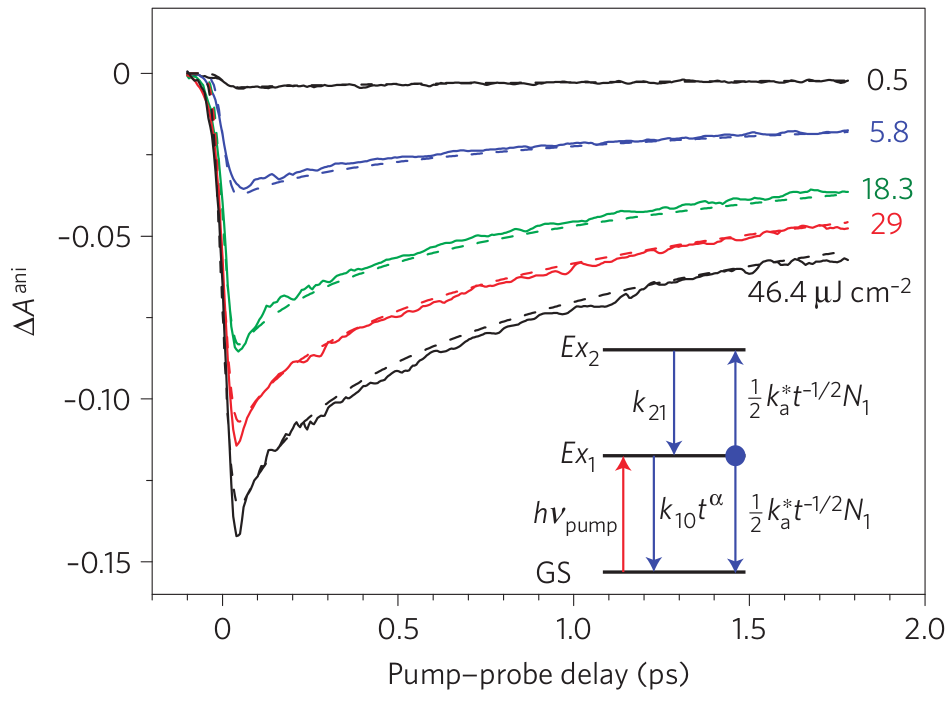
\includegraphics[scale=1.2]{images/chapter_prior_works/dtt_2_luer_2009}
	\caption{Differential absorption probed at the $E_{11}$ transition of (6,5) nanotubes presented with labeled pump fluences (\si{\micro \joule} \si{\cm^{-2}}). The pump and probe pulses were centered at wavelengths 960 and 992 nm respectively and were polarized parallel to each other. The dashed lines correspond to fits produced from the kinetic model shown in the inset. Here, excitons in first sub-band $E_{\text{x}_1}$ created by an optical pump of photon energy $h \nu_\text{pump}$ and undergo exciton-exciton annihilation at a time-dependent rate $k_\text{a}^* t^{-1/2}$ which creates a population of excitons in the second sub-band $E_{\text{x}_2}$. The variables $k_{21}$ and $k_{10}t^{\alpha}$ represent, respectively, decay rates from $E_{\text{x}_2}$ to $E_{\text{x}_1}$ and $E_{\text{x}_1}$ to the ground state. Reproduced from Ref.\ \cite{luer2009size}.}
	\label{fig:dtt_luer_2009}
\end{figure}


Fits of the model to the experimental data gave a time-dependent annihilation constant of $k_\text{a}(t) = 1.0 \times 10^7 \text{nm } \text{s}^{-1/2} \cdot \text{t}^{-1/2}$. However, Figure \ref{fig:dtt_2_luer_2009} demonstrates that Luer et al.\ did not observe strong evidence for efficient exciton-exciton annihilation. The normalized transient absorption curves do not appear to show a dominant early decay process that becomes drastically faster as the pump fluence increases.


Luer et al.\ also estimated size of excitons occuring in (6,5) SWCNTs using the well-known phase-space filling model \cite{schmitt1985theory, greene1990all}. According to this model, the relative change in oscillator strengths of excitonic resonances occurs as a result of the Pauli exclusion principle. Indeed, this change in the oscillator strength $\delta f_\text{}/ f_\text{}$ depends on the momentum-space, distribution functions $f_\text{e}(k)$ and $f_\text{h}(k)$ of electrons and holes respectively and is therefore written as
\begin{equation}
	\frac{\delta f_\text{}}{f_\text{}} = - \sum_{k} \left\{ \frac{ [ f_\text{e}(k) + f_\text{h}(k)] \tilde{\Psi}_\text{exc}(k)}{\Psi_\text{exc}(x=0)} \right\},
	\label{eq:osc_strength}
\end{equation}
which also includes the exciton wavefunction $\Psi_\text{exc}$ as well as its corresponding Fourier transform $\tilde{\Psi}_\text{exc}$.

\begin{figure}[ht]
	\centering
	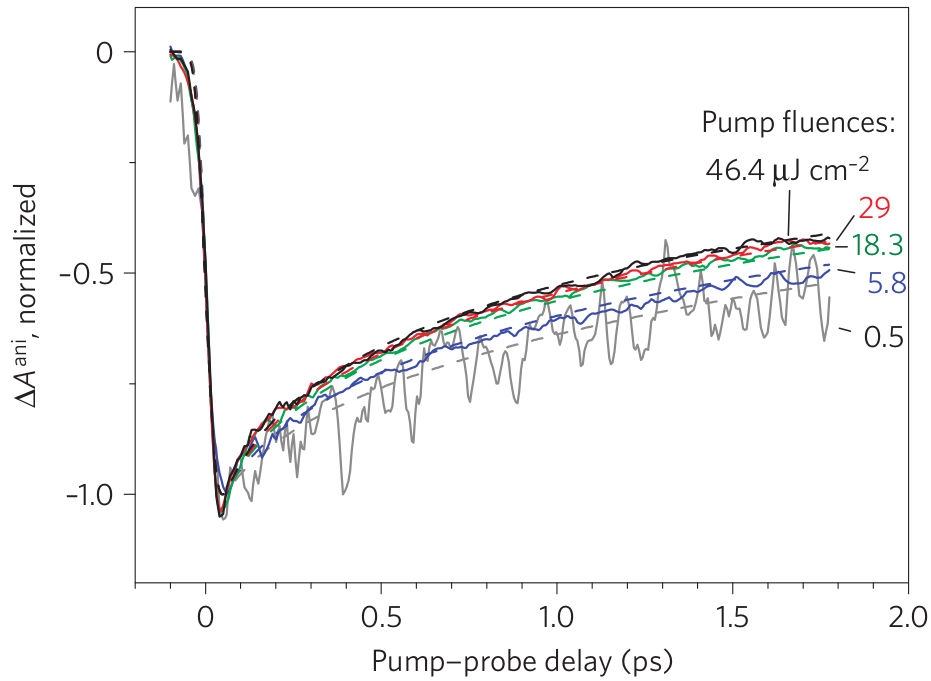
\includegraphics[scale=1.2]{images/chapter_prior_works/dtt_3_luer_2009}
	\caption{Normalized transient aborption data taken from Figure \ref{fig:dtt_luer_2009}. The relaxation dynamics do not appear to show a strong depdence on pump fluence. Hence, exciton-exciton annihilation is said to be an inefficient process in this scenario. Reproduced from Ref.\ \cite{luer2009size}.}
	\label{fig:dtt_2_luer_2009}
\end{figure}

For electrons and holes that pair together to form excitons, these the distribution functions are given as
%
\begin{equation}
	f_\text{e}(k) = f_\text{e}(k) = \frac{N}{2} | \tilde{\Psi}_\text{exc}(k)|^2,
\end{equation}
%
where $N$ refers to the density of excitons per unit length. In this expression, excitons represent a linear combination of single-particle, fermionic states distributed according to $\tilde{\Psi}_\text{exc}(k)$ \cite{schmitt1985theory}. Therefore, the formation of an exciton must correspond to an occupation probability in the fermion phase space $|\tilde{\Psi}_\text{exc}(k)|^2$ \cite{schmitt1985theory}. This probability is equally shared between spin-up and spin-down states which explains the factor of 1/2 \cite{schmitt1985theory}.

The exciton wavefunction $\Psi_\text{exc}$ can be approximated as
\begin{equation}
	\Psi_\text{exc}(x) = \left( \sqrt{a \sqrt{\pi}} \right)^{-1} \exp[-x^2 / (2 \xi^2_\text{e})],
\end{equation}
where $\xi_\text{e}$ represents the electron-hole correlation length, otherwise known as the exciton size \cite{capaz2006diameter}. Using this wavefunction, Equation \eqref{eq:osc_strength} becomes
%
\begin{equation}
	\frac{\delta f}{f} = - N \gamma \xi_\text{e}, \hspace{4mm} \gamma \approx 2.05.
\end{equation}
%
Here, $\gamma$ is a proportionality constant that varies with the wavefunction used to perform this calculation. Certainly, the relative change in the oscillator strength is related to the differential absorption $\Delta A / A$ as well as a saturation density $N_\text{s}$ by the expression
\begin{equation}
	\frac{\delta f}{f} = \frac{\Delta A}{A} = \frac{N}{N_\text{s}},
\end{equation}
where $N_\text{s}^{-1} = \gamma \xi_\text{e}$.
\begin{equation}
	\Delta A = -r_\text{a} \gamma \sigma_\text{C} \frac{\xi_\text{e}}{\xi_\text{C}} I_\text{abs}
	\label{eq:abs_exc_len}
\end{equation}

\begin{figure}[ht]
	\centering
	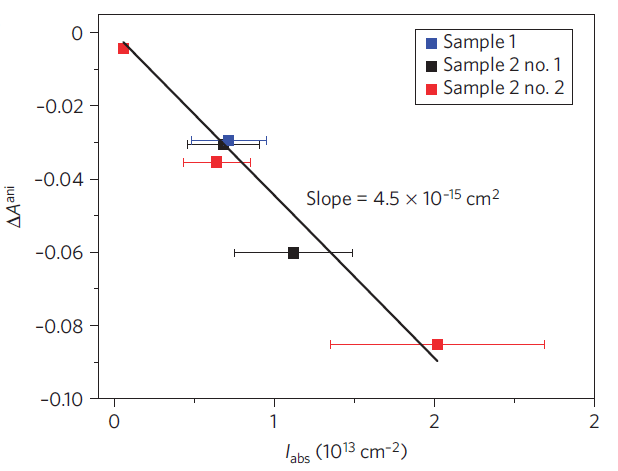
\includegraphics[scale=0.8]{images/chapter_prior_works/exciton_size_fit_luer_2009}
	\caption{Maximum differential absorption as a function of the absorbed pump fluence $I_\text{abs}$. The solid line represents a linear regression using function defined in Equation \eqref{eq:abs_exc_len} which was used to obtain an exciton size of $\xi_\text{e} = 2.0 \pm 0.7$ nm. Reproduced from Ref.\ \cite{luer2009size}.}
	\label{fig:lin_fit_luer_2009}
\end{figure}

{\color{red}UNFINISHED } Figure \ref{fig:lin_fit_luer_2009} shows results of fitting. Get exciton size of $2.0 \pm 0.7$ nm which agrees with theory \cite{tretiak2007excitons}. From Equation \eqref{eq:exc_anih_diffuse_luer_2009}, obtain a diffusion length less than 10 nm which happens to be an order of magnitude less than the corresponding value obtained in fluorescence measurements \cite{cognet2007stepwise}. These results, combined with weak exciton-exciton annihilation, lead Luer et al.\ to conclude that differential absorption probes total population of excitons, many of which short-lived and do not directly participate in exciton-exciton annihilation due to shorter diffusion lengths. However, time-resolved fluoresence measurements probe long-lived excitons that have higher diffusion lengths and are therefore more likely to engage in exciton-exciton annihilation processes.



\subsection{Murakami et al.\ (2009)}
{\color{red} UNFINISHED} Efficient exciton-exciton annihilation \cite{murakami2009existence}.




%\section{Possible Presence of Bi-excitons and Trions}

%non-degenerate pump-probe. Amplified Ti:sapphire laser operating at 200 KHz and pulse duration of 100 fs. Probe generated using supercontinuum generation in a sapphire crystal. Pump generated using optical parametric amplifier (OPA). Studied a (6,5)-enriched dispersion. Figure \ref{fig:abs_yuma} shows linear absorption spectrum of sample.

%\begin{figure}[ht]
%	\centering
%	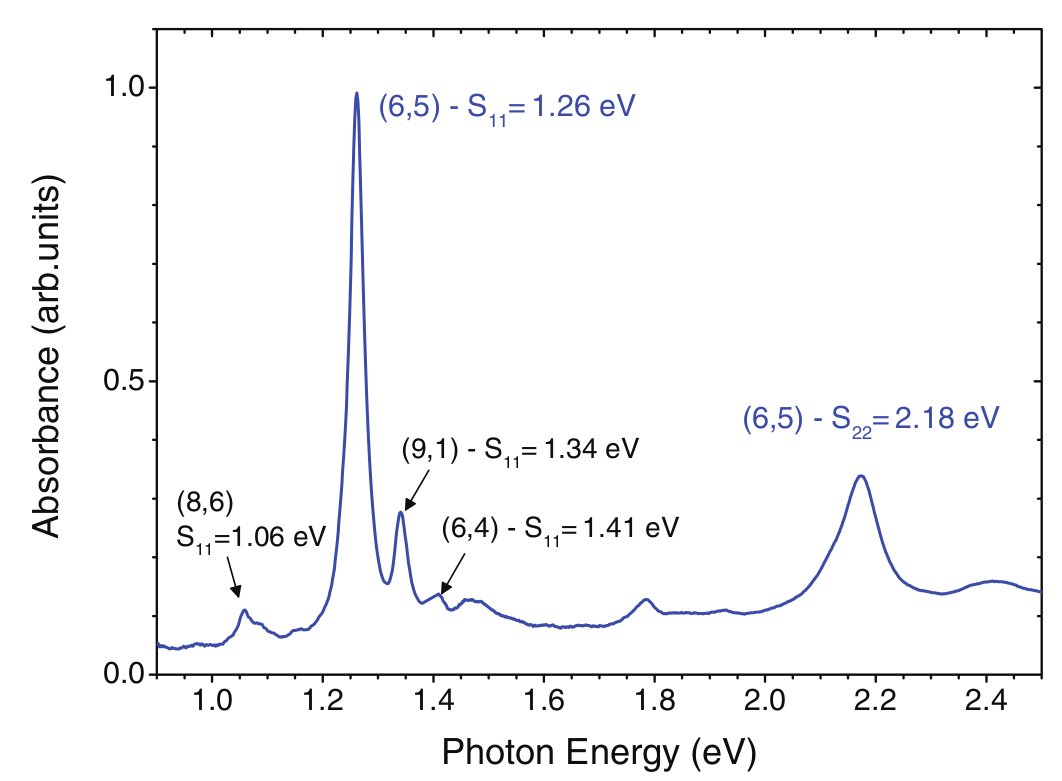
\includegraphics[scale=0.3]{images/chapter_prior_works/abs_yuma}
%	\caption{Slightly different nomenclature. Here, $S_\text{ij} \equiv E_\text{ij}$.  Reproduced from Ref.\ \cite{yuma2013biexciton}.}
%	\label{fig:abs_yuma}
%\end{figure}

%Figure \ref{fig:dtt_yuma} shows experimental data after resonantly exciting $E_{22}$ transition of (6,5) nanotube. Notice photo-bleaching and a blue shift occuring at $E_{11}$ peak. Interpreted as excitons occupying $E_{11}$ states. Charge screening due to Coulomb interactions between excitons blueshifts exciton peak. State that initial sharp decay due to exciton-exciton annihilation.

%Observed photo-induced absorption at 1.13 eV. Attribute this to the formation of biexcitons. Provided additional evidence by pumping at and below $E_{11}$. When pumping below $E_{11}$, photo-induced absorption at 1.13 eV recedes. When pumping $E_{11}$ resonantly, photo-induced absorption becomes more significant indicating that it may be directly associated with (6,5). Carrier dynamics at $E_{11}$ and bi-exciton appear to be correlated with each other.

%\begin{figure}[ht]
%	\centering
%	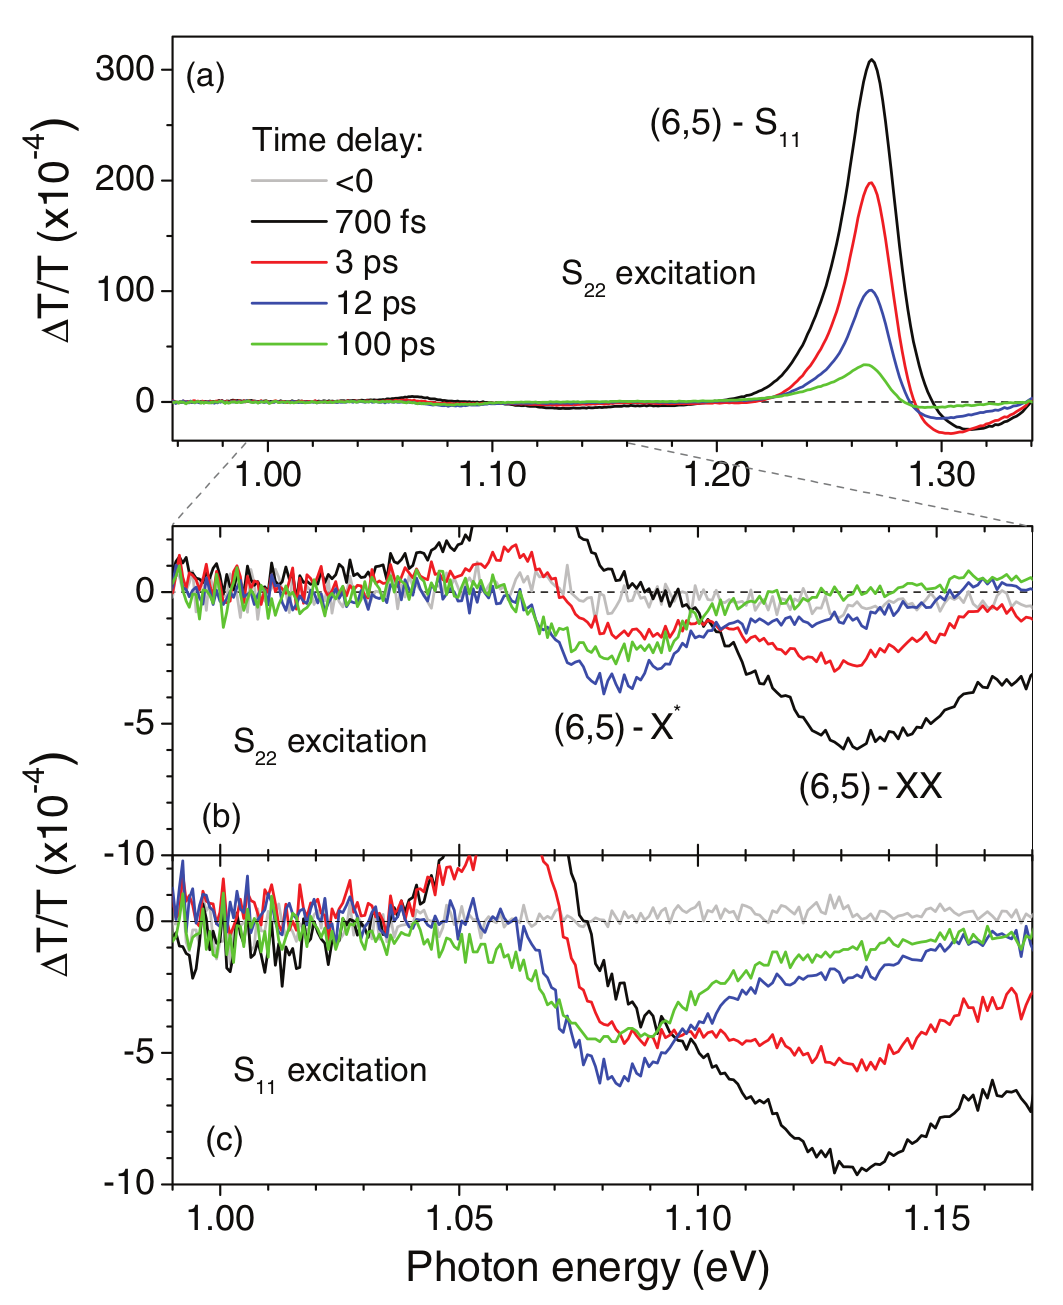
\includegraphics[scale=0.3]{images/chapter_prior_works/dtt_yuma}
%	\caption{{\color{red} UNFINISHED} Reproduced from Ref.\ \cite{yuma2013biexciton}.}
%	\label{fig:dtt_yuma}
%\end{figure}


%Exciton-Exciton annihilation \cite{valkunas2006exciton, yuma2013biexciton}.
%They also show that exciton-exciton annihilation occurs over a time scale such that it is hard to reach Mott densitty of excitons where excitons immediately dissociate to form plasma of free carriers. These a
%Apparently, excitons dissociate into free electron-hole pairs before recombination occurs \cite{kumamoto2014spontaneous}.

\newpage

\section{The Optical Stark Effect}
{\color{red} UNFINISHED}

\subsection{Song et al.\ (2006)}
Ref.\ \cite{song2006optical}.

\subsection{Maeda et al.\ (2006)}

\begin{figure}[ht]
	\centering
	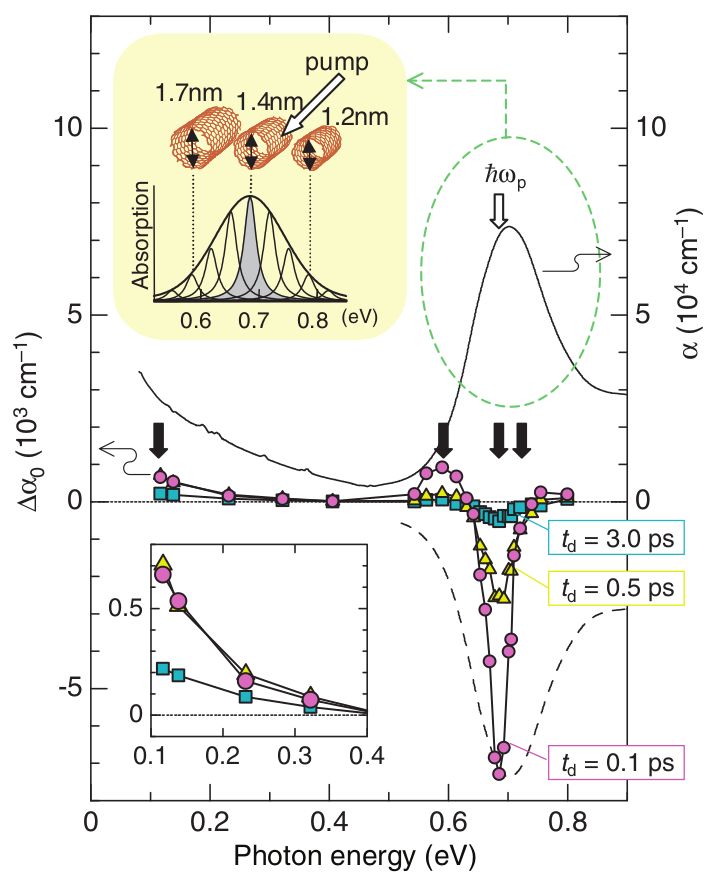
\includegraphics[scale=0.4]{images/chapter_prior_works/stark_shift_maeda}
	\caption{{\color{red} UNFINISHED} Reproduced from Ref.\ \cite{maeda2006gigantic}.}
\end{figure}

\subsection{Matsumoto et al.\ (2006)}

Ref.\ \cite{matsumoto2006optical}.

\subsection{Tao et al.\ (2009)}

Ref. \cite{tao2009subpicosecond}.

\section{Discussion}


Conflicting reports of exciton-exciton annihilation. Consensus regarding efficiency of exciton exciton isn't so clear. There could be a number of reasons for disagreements in each work. These can include, type of sample studied, power density of the optical pump as well as pump wavelength. Samples in early studies used HiPCo or CoMoCAT dispersions which contained several different chiralities. As noted by Ostojic et al.\ (2004), optical excitations can cause both resonant and non-resonant excitations in the ensemble. Moreover, multi-photon processes occuring in metallic nanotubes, which have resonances at higher photon energies, could also play a role.

Exciton sizes can vary depending on dielectric environment \cite{mann201613}.

One question: Do carrier relaxation processes differ when exciting resonantly or nonresonantly? If so, how?

Does phonon side-band play a role here? It has been ignored in early studies as $E_{11}$ and $E_{22}$ resonance are dominant in optical absorption spectrum.
Wang et al (2004) pumped at 810 nm which is right between $E_{11}$ and $E_{22}$ of many of the semiconducting in their sample.

Dielectric environment can have an effect on
